\chapter{UML diagramy a obrázky}
\section{Use cases}
\label{use_cases}

\begin{figure}[H]
\begin{center}
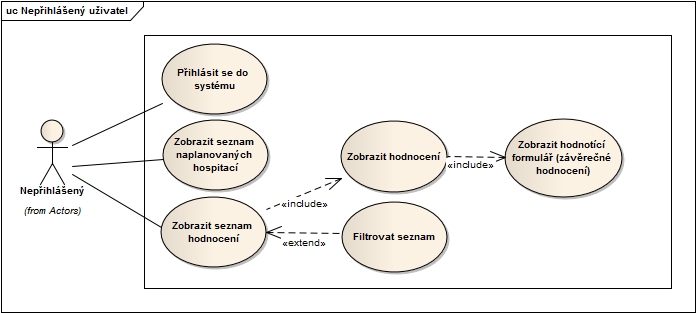
\includegraphics[width=12cm]{figures/actor_base}
\caption{Use case - nepřihlášený uživatel}
\label{fig:actor_base}
\end{center}
\end{figure}

\begin{figure}[H]
\begin{center}
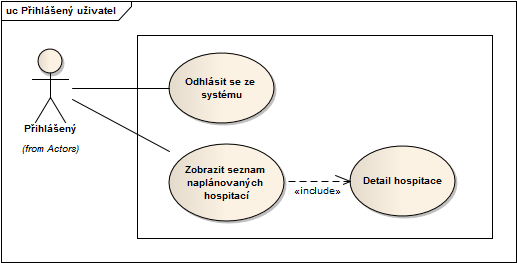
\includegraphics[width=12cm]{figures/actor_logged}
\caption{Use case - přihlášený uživatel}
\label{fig:actor_logged}
\end{center}
\end{figure}

\begin{figure}[H]
\begin{center}
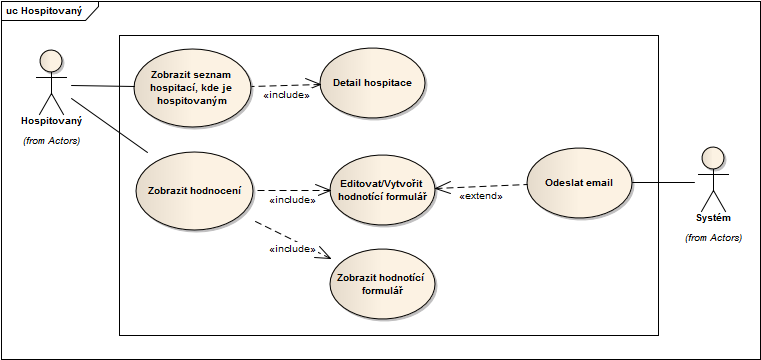
\includegraphics[width=12cm]{figures/actor_observed}
\caption{Use case - hospitovaný}
\label{fig:actor_observed}
\end{center}
\end{figure}

\begin{figure}[H]
\begin{center}
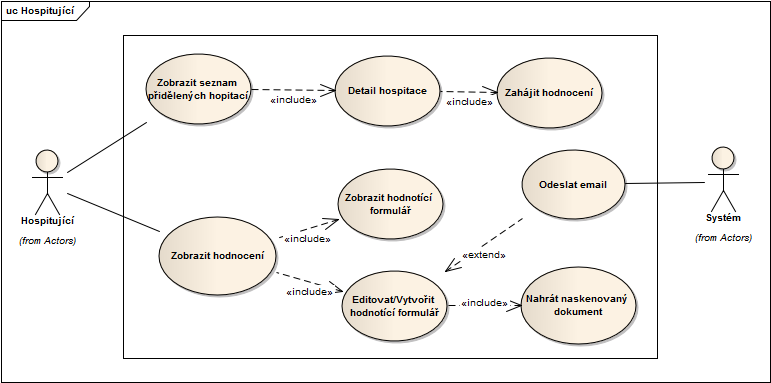
\includegraphics[width=12cm]{figures/actor_observer}
\caption{Use case - hospitující}
\label{fig:actor_observer}
\end{center}
\end{figure}

\begin{figure}[H]
\begin{center}
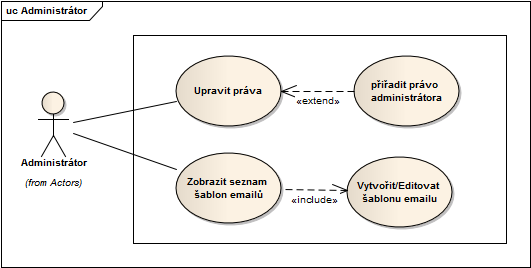
\includegraphics[width=12cm]{figures/actor_root}
\caption{Use case - administrátor}
\label{fig:actor_root}
\end{center}
\end{figure}

\begin{figure}[H]
\begin{center}
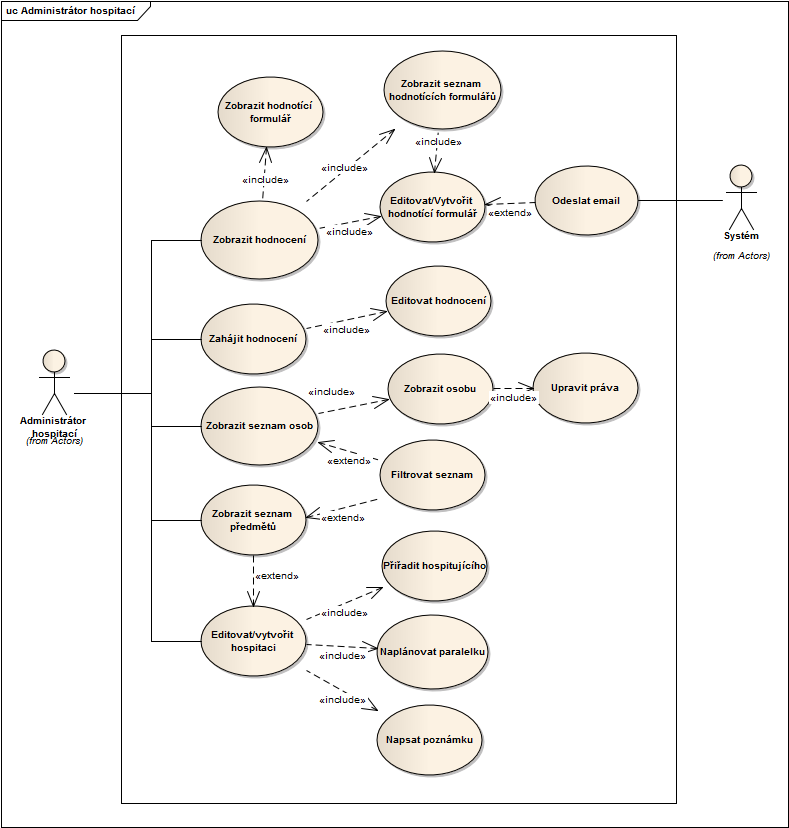
\includegraphics[width=14cm]{figures/actor_admin}
\caption{Use case - administrátor hospitací}
\label{fig:actor_admin}
\end{center}
\end{figure}


\chapter{Dynamické formuláře}
\label{sec:forms}
\begin{table}[h]
\begin{center}
\begin{tabular}{|l|c|l|}

\hline
\textbf{Typ} & \textbf{Návratová hodnota} & \textbf{Popis} \\ \hline
label &  & textový popisek \\\hline
integer & číslo & vstupní element pro čísla \\ \hline
text & text & formulář pro psaní textů \\\hline
text/file & text & formulář pro psaní textů s možností \\ & &  nahrání souboru s naskenovaným formulářem \\\hline
ranking\_table &  & tabulka pro hodnocení, může obsahovat několik \\ & & elementů typu \textit{ranking} \\\hline
column\_table & & tabulka do které se vkládají jiné elementy \\ & &  po sloupcích \\\hline
ranking & [A,B,C,D,E,F] & vstupní element pro zadávání známek \\ & &   od A do F \\\hline
ranking\_scale & & tabulka s hodnotící stupnicí \\\hline
note & text & vstupní element pro zápis textové poznámky \\\hline

\end{tabular}
\caption{Seznam podporovaných typů elementů}
\label{tab:elements}
\end{center}
\end{table}

\begin{figure}[H]
\begin{center}
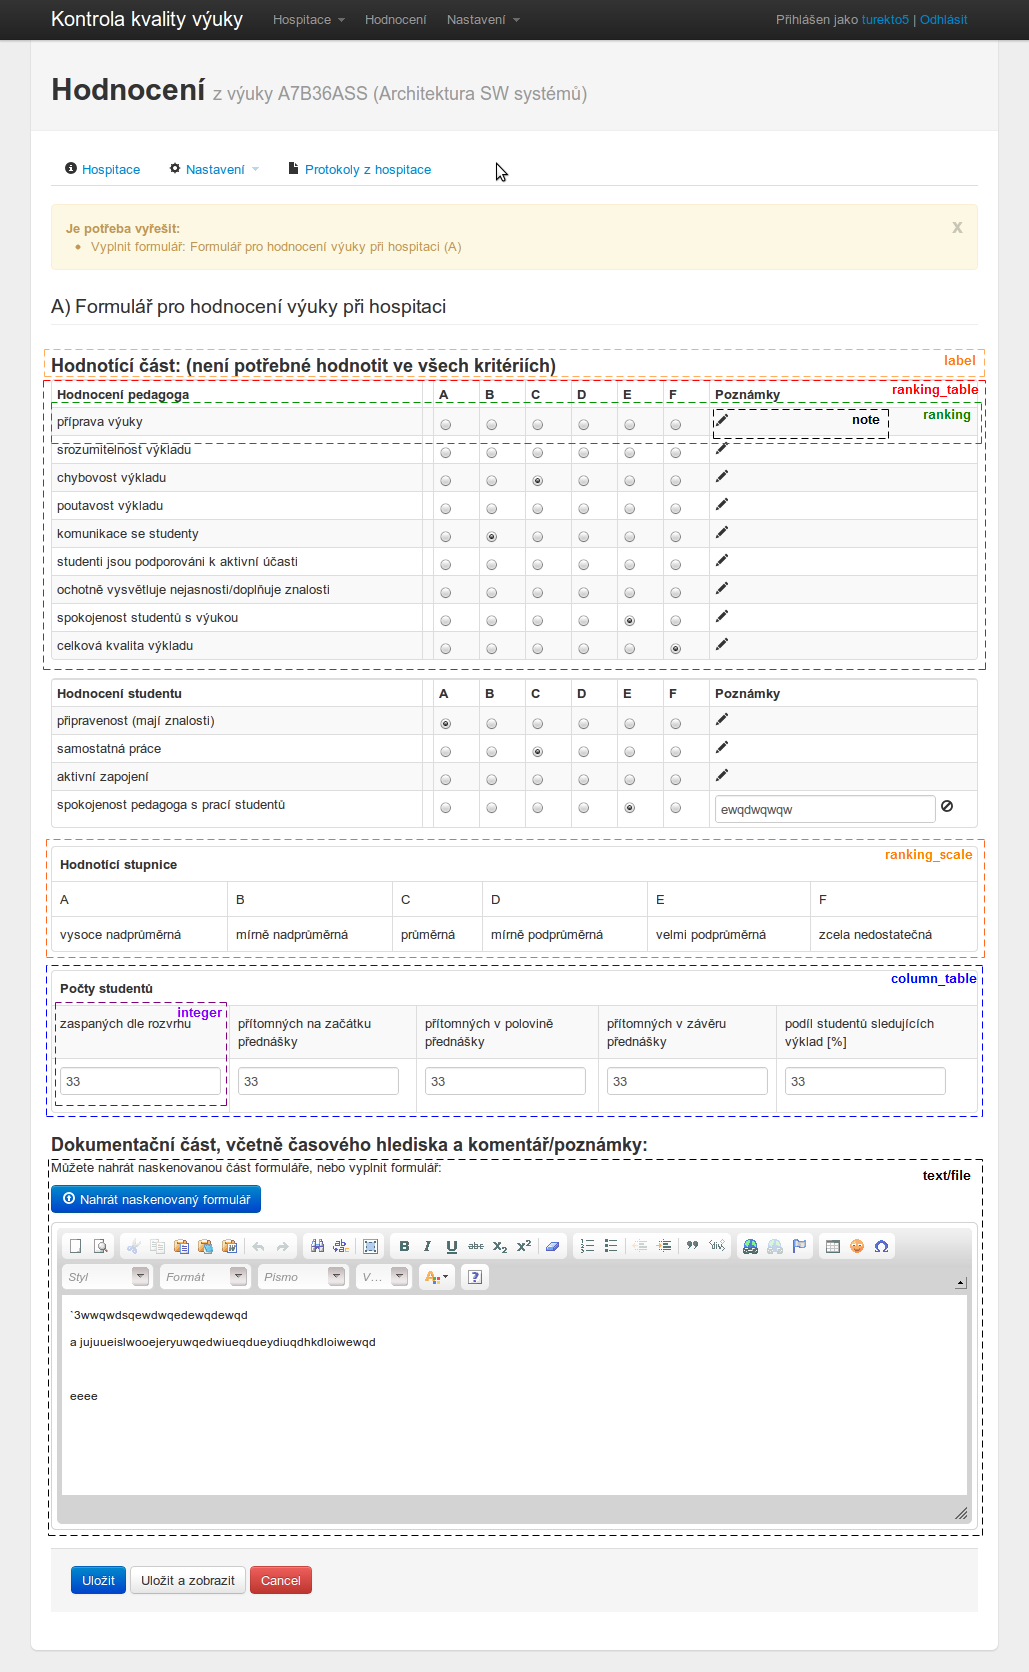
\includegraphics[width=14cm]{figures/form_A}
\caption{Hodnotící formulář A}
\label{fig:form_a}
\end{center}
\end{figure}

\chapter{Test Cases}
\label{test}
\begin{description}
\item[Test Case ID:] 1
\begin{description}
\item[Co:] Přihlášení uživatele do systému.
\item[Role:] Nepřihlášený uživatel
\item[Požadavky:] Musí být zprovozněna služba FELid.
\item[Očekávaný výsledek:] Uživatel je přihlášený.
\end{description}
\end{description}

\begin{description}
\item[Test Case ID:] 2
\begin{description}
\item[Co:] Odhlášení uživatele ze systému.
\item[Role:] Přihlášený uživatel
\item[Požadavky:] Musí být zprovozněna služba FELid.
\item[Očekávaný výsledek:] Uživatel není přihlášený.
\end{description}
\end{description}

\begin{description}
\item[Test Case ID:] 3
\begin{description}
\item[Co:] Seznam naplánovaných hospitací.
\item[Role:] Všechny
\item[Očekávaný výsledek:] Zobrazil se seznam naplánovaných hospitací a obsahuje všechny hospitace typu ohlášená a plovoucí.
\end{description}
\end{description}

\begin{description}
\item[Test Case ID:] 4
\begin{description}
\item[Co:] Seznam hodnocení s filtrováním dle: předmětu, učitele, garanta a semestru.
\item[Role:] Všechny
\item[Požadavky:] Existují hodnocené hospitace.
\item[Očekávaný výsledek:] Zobrazil se seznam a lze v něm filtrovat záznamy. 
\end{description}
\end{description}

\begin{description}
\item[Test Case ID:] 5
\begin{description}
\item[Co:] Přístup k formuláři Závěrečné hodnocení hospitace.
\item[Role:] Všechny
\item[Požadavky:] Existuje ukončená hospitace.
\item[Očekávaný výsledek:] Zobrazil se formulář. 
\end{description}
\end{description}

\begin{description}
\item[Test Case ID:] 6
\begin{description}
\item[Co:] Seznam hospituji.
\item[Role:] Hospitující
\item[Očekávaný výsledek:] Zobrazil se seznam a jsou v něm všechny hospitace, které uživatel hospituje v daném semestru.
\end{description}
\end{description}

\begin{description}
\item[Test Case ID:] 7
\begin{description}
\item[Co:] Zahájení hodnocení hospitace.
\item[Role:] Hospitující a administrátor hospitací
\item[Požadavky:] Naplánovaná hospitace
\item[Očekávaný výsledek:] Bylo úspěšně zahájeno hodnocení.
\end{description}
\end{description}

\begin{description}
\item[Test Case ID:] 8
\begin{description}
\item[Co:] Vyplnit hodnotící formulář A
\item[Role:] Hospitující
\item[Požadavky:] Zahájené hodnocení hospitace
\item[Očekávaný výsledek:] Hodnotící formulář byl úspěšně uložen.
\end{description}
\end{description}

\begin{description}
\item[Test Case ID:] 9
\begin{description}
\item[Co:] Nahrát přílohu k hodnotícímu formuláři A
\item[Role:] Hospitující
\item[Požadavky:] Vyplněný formulář A
\item[Očekávaný výsledek:] Příloha je uložená a lze ji stáhnout.
\end{description}
\end{description}

\begin{description}
\item[Test Case ID:] 10
\begin{description}
\item[Co:] Vyplnit hodnotící formulář B
\item[Role:] Hospitující
\item[Požadavky:] Zahájené hodnocení hospitace, vyplněné všechny formuláře A
\item[Očekávaný výsledek:] Hodnotící formulář byl úspěšně uložen.
\end{description}
\end{description}

\begin{description}
\item[Test Case ID:] 11
\begin{description}
\item[Co:] Vyplnit hodnotící formulář C
\item[Role:] Hospitovaný
\item[Požadavky:] Zahájené hodnocení hospitace, vyplněný formulář B
\item[Očekávaný výsledek:] Hodnotící formulář byl úspěšně uložen.
\end{description}
\end{description}

\begin{description}
\item[Test Case ID:] 12
\begin{description}
\item[Co:] Vyplnit hodnotící formulář D
\item[Role:] Hospitující
\item[Požadavky:] Zahájené hodnocení hospitace, vyplněný formulář B
\item[Očekávaný výsledek:] Hodnotící formulář byl úspěšně uložen a hospitace je ve stavu ukončená.
\end{description}
\end{description}

\begin{description}
\item[Test Case ID:] 13
\begin{description}
\item[Co:] Odesílání emailů po uložení hodnotícího formuláře.
\item[Role:] Systém
\item[Požadavky:] Existuje emailová šablona pro druh hodnotícího formuláře.
\item[Očekávaný výsledek:] Email byl správně sestavený a doručený do emailové schránky.
\end{description}
\end{description}

\begin{description}
\item[Test Case ID:] 14
\begin{description}
\item[Co:] Seznam hospitován.
\item[Role:] Hospitovaný
\item[Očekávaný výsledek:] V seznamu jsou všechny hospitace, které mají zahájené hodnocení a uživatel je s nimi ve vztahu hospitovaný.
\end{description}
\end{description}

\begin{description}
\item[Test Case ID:] 15
\begin{description}
\item[Co:] Vytvořit hospitaci
\item[Role:] Administrátor hospitací
\item[Očekávaný výsledek:] Hospitace byla uložena.
\end{description}
\end{description}

\begin{description}
\item[Test Case ID:] 16
\begin{description}
\item[Co:] Přiřadit hospitujícího k hospitaci
\item[Role:] Administrátor hospitací
\item[Požadavky:] Existuje vytvořená hospitace, kterou uživatel spravuje.
\item[Očekávaný výsledek:] K hospitaci byl úspěšně přiřazen hospitující.
\end{description}
\end{description}

\begin{description}
\item[Test Case ID:] 17
\begin{description}
\item[Co:] Naplánovat hospitaci
\item[Role:] Administrátor hospitací
\item[Požadavky:] Existuje vytvořená hospitace, kterou uživatel spravuje.
\item[Očekávaný výsledek:] Hospitace je ve stavu naplánovaná.
\end{description}
\end{description}

\begin{description}
\item[Test Case ID:] 18
\begin{description}
\item[Co:] Napsat poznámku k hospitaci
\item[Role:] Administrátor hospitací
\item[Požadavky:] Existuje vytvořená hospitace, kterou uživatel spravuje.
\item[Očekávaný výsledek:] Poznámka byla vytvořena a lze ji zobrazit.
\end{description}
\end{description}

\begin{description}
\item[Test Case ID:] 19
\begin{description}
\item[Co:] Přiřadit roli osobě
\item[Role:] Administrátor
\item[Očekávaný výsledek:] Osobě byla úspěšně přiřazena role.
\end{description}
\end{description}


%*****************************************************************************
\chapter{Instalační a uživatelská příručka}
Instalační příručka je napsaná pro zprovoznění aplikace v prostředí development. Návod je určený pro operační systém Ubuntu 11.10. Pro zprovoznění aplikace musíme nainstalovat tyto programy:
\begin{itemize}
\item Ruby 1.9.3
\item RubyGems 1.8.13
\item Ruby on Rail 3.2.1
\item Databázový systém Mysql 5.5 nebo SQLite 3
\item Git
\end{itemize}

\section{Instalace}
Nejprve je potřeba nainstalovat platformu Ruby do systému. S ruby nainstalujte i balík build-essential a git-core kvůli  knihovnám, které jsou potřeba pro zprovoznění aplikace. 

\begin{verbatim}
sudo apt-get install ruby1.9.3-full build-essential git-core
\end{verbatim}

Dále nainstalujte balíčkovací systém RubyGems a aktualizujte ho na poslední podporovanou verzi.
\begin{verbatim}
sudo apt-get install rubygems1.8
sudo gem update --system
\end{verbatim}

V poslední fázi je potřeba nainstalovat Ruby on Rails pomocí balíčkovacího programu rubygems.

\begin{verbatim}
sudo gem install rails
\end{verbatim}

Po nainstalování Ruby on Rails je potřeba doinstalovat všech závislosti aplikace. Nejprve musíme někam do systému zkopírovat aplikaci např. do domovského adresáře. Ve všech dalších krocích se budeme pohybovat v adresáři aplikace. Druhý příkaz slouží k instalaci závislostí aplikace.

\begin{verbatim}
cd ~/Hospitace
bundle install
\end{verbatim}  

\section{Konfigurace a příprava aplikace}
Před spuštěním aplikace je důležité nastavit přístupové údaje k databázi. Nastavení databáze se nachází v souboru config/database.yml, který se nalézá v aplikaci. Pro zavedení databáze pak stačí jen spustit příkazy:

\begin{verbatim}
rake db:create
rake db:migrate
\end{verbatim}  

Máme vytvořenu databázi, je nutné ji naplnit naplnit daty z KOSapi. Pro tento účel slouží příkaz:

\begin{verbatim}
rake import
\end{verbatim}

\section{Spuštění aplikace}
Pro spuštění aplikace použijte webový server Webrick, který je součástí Ruby on Rails. Po spuštění bude aplikace běžet na portu 3000.
Příkaz pro spuštění:
 
\begin{verbatim}
rails server
\end{verbatim}

%*****************************************************************************
\chapter{Obsah přiloženého CD}
\begin{figure}[h]
	\dirtree{%
		.1 /.
		.2 EA/.
		.3 hospitace.ear\DTcomment{analýza aplikace v programu Enterprise Architect}.
		.2 prototyp/\DTcomment{prototyp aplikace}.
		.3 src/\DTcomment{zdrojové kódy prototypu}.
		.3 BP.pdf\DTcomment{text prototypu ve formátu PDF}.
		.2 src/\DTcomment{zdrojové kódy aplikace}.
		.2 text/.
		.3 thesis.pdf\DTcomment{text práce ve formátu PDF}.
		.2 thesis/\DTcomment{zdrojová forma práce ve formátu
\LaTeX{}}.
 		.3 figures/\DTcomment{obrázky pro text práce}.
		.2 readme.txt\DTcomment{stručný popis obsahu CD}.
	}
	\caption{Obsah CD}
\label{tree:obsah_cd}
\end{figure}
%$ tree . >tree.txt
